\documentclass{IEEEtran}
\usepackage[utf8]{inputenc}
\usepackage[T1]{fontenc}
\usepackage[ngerman]{babel}
\usepackage{acronym}
\usepackage{footnote}
\usepackage{algorithmic}
\usepackage{graphicx}
\usepackage[autostyle=true,german=quotes]{csquotes}
\usepackage{gensymb}
\usepackage{eurosym}
\usepackage{booktabs}
\usepackage{array}
\usepackage{todonotes}
\usepackage{microtype}
\usepackage{icomma}


\usepackage{hyperref}

\long\def\comment / *#1* /{}



% -----------------------------------------------------------------------------
% Visible TODO and FIXME markers
% -----------------------------------------------------------------------------
\newcounter{TODOCOUNT}
\newcommand{\TODO}[1]{\vspace{0.5em}\todo[inline, color=orange]{#1}\stepcounter{TODOCOUNT}}
\newcommand{\FIXME}[1]{\todo[size=\small, color=red]{#1}\stepcounter{TODOCOUNT}}
\AtEndDocument{
	\ifnum\value{TODOCOUNT}>0
		%\cleardoublepage
		\listoftodos
	\fi
}
% -----------------------------------------------------------------------------


\newcolumntype{x}[1]{>{\centering\arraybackslash\hspace{0pt}}p{#1}}



\begin{document}


\title{cowbusconfig -- Ansatz zur dezentralen Konfiguration von Gebäudeautomation}
\author{Patrick~Kanzler \and Michael~Zapf}
\date{\today}



\maketitle

\begin{abstract}
    Um die Vorzüge intelligenter Haussteuerung einer breiten Masse zugänglich
    zu machen, müssen die System einfach handhabbar werden.
    Besonders die Konfiguration, also die Zuordnung von Sensorevent zu
    Schaltaktion, muss einfach durchführbar und ebenso einfach anpassbar
    bzw. revidierbar sein. Diese Arbeit schlägt einen Ansatz vor,
    der in einem dezentralen Sensor-Aktor-Netzwerk eine einfache
    Konfigurationsmöglichkeit bieten soll.
    Dabei erfolgt die eigentliche Konfiguration per Webbrowser und kann
    jederzeit wieder ausgelesen, geändert und ergänzt werden.
\end{abstract}

\section{Einleitung}
    \enquote{Smart Home} ist ein Schlagwort, um das man im 21. Jahrhundert
    kaum noch herum kommt. Der moderne Mensch möchte sein Zuhause vernetzen.
    Vor allem in gewerblich genutzten Gebäuden ist es inzwischen üblich,
    auf die in der Vergangenheit übliche harte Verdrahtung von Sensoren und
    Aktoren -- sprich zum Beispiel Lichtschalter und Leuchte -- zu verzichten
    und auf intelligente Einzelkomponenten zu setzen, die meist in einer
    Bustopologie verbunden sind. Der Vorteil liegt auf der Hand:
    Durch das Fehlen der festen Zuordnung zwischen Auslöser
    (\emph{Lichtschalter gedrückt}) und Wirkung (\emph{Leuchte A an})
    können softwarebasiert Ursache-Wirkung-Beziehungen modelliert, evaluiert
    und korrigiert werden.

    Etablierte Systeme setzen dabei in der Regel auf eine
    Konfigurationssoftware, in der die teils komplexen Kommunikation- und
    Schaltvorgänge modelliert werden.
    Die einzelnen an den Bus angeschlossenen Komponenten werden häufig nur
    mit dem logischen Endergebnis konfiguriert,
    aus dem sich die ursprünglichen Absichten nicht mehr vollständig ableiten
    lassen.

    In dieser Arbeit beschäftigen wir uns mit dem Gedanken,
    Teilnehmer in einem Gebäudeautomationsnetzwerk so konfigurierbar zu gestalten,
    dass die Konfiguration jederzeit mit minimalen Aufwand auslesbar
    und änderbar ist.
    Die Idee ist im Kontext eines DIY-Projektes entstanden und zielt deshalb
    auch einfachste Anforderungen ab.

\section{Verwandte Arbeiten}
    Gebäudeautomation wird inzwischen sowohl in der Praxis
    als auch in der Forschung erprobt. Hierbei konkurrieren verschiedene Systeme
    und Technologien, denen unterschiedlichste Paradigmen zugrunde liegen.
    Zur Veranschaulichung möchten wir hier ein System aus der Praxis betrachten,
    das auf dezentraler Kommunikation beruht,
    sowie einen Ansatz aus der Forschung,
    der einen zentralen Kommunikationsserver vorschlägt.

    \subsection{Europäischer Installationsbus (EIB) / KNX}
    Der unter der Abkürzung EIB bekannte Europäische Installationsbus
    ist ein offener Standard und nach subjektivem Empfinden das in der Praxis
    wohl meistgenutzte System in der Gebäudeautomation.
    Inzwischen wird er unter dem Namen KNX entwickelt und vertrieben.
    Es sind weltweit fast 7000 Produkte auf dem Markt \cite{knx-prod}, die
    mit einer Twisted-Pair-Leitung verbunden werden
    (weitere Medien -- auch drahtlose -- sind verfügbar),
    über die Nachrichten direkt untereinander ausgetauscht werden.
    \cite{knx-trans}

    Die Konfiguration der Schaltregeln etc. erfolgt nach der Installation
    der Komponenten durch einen Fachmann mithilfe von Software aus der
    ETS-Familie. Dabei handelt es sich um proprietäre Software,
    die von der KNX Association\footnote{\url{http://www.knx.org/}} entwickelt
    und vertrieben wird.
    \cite{knx}

    KNX eignet sich besonders im Bereich großer Gebäude, in denen die
    elektrischen Systeme von einem Fachmann geplant, installiert und auch über
    Jahre hinweg gewartet werden. Ein entscheidender Nachteil von KNX ist,
    dass die Konfiguration, sobald sie einmal in die Steuergeräte geschrieben
    ist, nicht mehr ohne weiteres ausgelesen werden kann.
    Um die Konfiguration zu ändern (um zum Beispiel neue Komponenten einzufügen
    oder auch nur eine einfache Schaltregel anzupassen) wird jedes mal
    die ursprünglich erstellte Projektdatei aus der ETS-Software benötigt.

    \subsection{zentrale skriptbasierte Steuerung}
        T. Haenselmann et al. beschreiben ein zentrales System, das weitgehend
        unabhängig von dem verwendeten Transportmedium ist.
        Sie schlagen eine drahtlose Kommunikation vor,
        der Kerngedanke jedoch, auf den wir uns hier beziehen werden,
        gilt jedoch medienunabhängig.
        Der grundlegende Ansatz besteht in der Einrichtung eines zentralen
        Servers, bei dem alle Nachrichten des Systems zusammenlaufen.
        Sensoren melden ihre Messwerte an diesen, der dann Schaltnachrichten
        an die Aktoren sendet.
        Die Entscheidung, welche Aktionen ausgelöst werden, trifft der Server
        mithilfe von Skripten, die der Benutzer hinterlegt.
        Diese Skripte können auch über eine Weboberfläche erstellt und
        verwaltet werden.
    \cite{haenselmann2007skriptbasierte}

    %\cite{drossos2013ansteuerung}
    %\cite{kuntz6servicecast}
    %\cite{kuntz2011dienstbasierte}

\section{Ansatz}
    Inspiriert von Haenselmann et al.s Arbeit möchten wir ein System vorschlagen,
    das ebenso über eine einfache Weboberfläche konfiguriert werden kann.
    Der Benutzer kann dort einfache Wenn-Dann-Regeln anlegen, bearbeiten und
    löschen, die das Verhalten der Aktoren in Abhängigkeit von Sensorereignissen
    festlegen.

    Der grundlegende Unterschied im Ansatz besteht jedoch darin,
    dass wir auf eine zentrale Kommunikationseinheit verzichten.

    \subsection{Voraussetzungen, Annahmen}
        Wir gehen davon aus, dass uns ein paketvermitteltes Netz vorliegt,
        in dem alle Teilnehmer eindeutig adressierbar sind.

        Als Test- und Referenzumgebung dient uns der \emph{cowbus}.
        Dabei handelt es sich um ein studentisches Projekt,
        das sich zum Ziel gesetzt hat,
        eine kostengünstige und einfach nachzubauende Plattform zu schaffen,
        die einen Einstieg in den Arbeits- und Forschungsbereich des
        \enquote{Smart Home} bzw. \enquote{Connected Home} ermöglichen soll.
        Der Nachrichtenaustausch erfolgt dabei drahtlos über eine
        $2,4$\,GHz-Funkverbindung. \cite{cowbus}

        Das Testnetzwerk besteht aus drei Komponenten:
        \begin{itemize}
            \item Als \textbf{Sensor} dient ein einfacher Taster.
                Er soll Schaltaktionen im Netzwerk auslösen.
            \item Eine LED dient als \textbf{Aktor},
                der beliebige Schaltaktionen im Netzwerk symbolisch darstellt.
            \item Zur \textbf{Konfiguration} der Geräte befindet sich
                außerdem ein
                Raspberry Pi\footnote{\url{http://www.raspberrypi.org}}
                im Netzwerk.
                Er wurde um ein Funkmodul erweitert und stellt eine
                Weboberfläche zur Verfügung,
                über die die Konfiguration ermöglicht werden soll.
                Außerdem ermöglicht er die \textbf{Überwachung} des Netzwerkverkehrs.
        \end{itemize}

    \subsection{Idee}
        Da \textbf{Sensoren} häufig höhere Anforderungen an den Energieverbrauch
        stellen, sollen sie in dem System \enquote{dumm} sein.
        Sie erarbeiten sich also kein Wissen über die anderen Netzwerkkomponenten
        und reagieren nicht, sondern agieren ausschließlich.
        Das ermöglicht uns sie die meiste Zeit in Energiesparmodi zu betreiben
        und nur dann aufzuwecken, wenn sie selbst ein Ereignis auslösen,
        zum Beispiel wenn der Benutzer einen Taster betätigt.

        \textbf{Aktoren} hingegen sind häufig mit stabilen Energiequellen
        ausgestattet, da sie meist gewisse Lasten schalten.
        Als Beispiele wären Leuchten, Jalousiemotoren oder auch Ventilatoren
        zu nennen.
        Daher bietet es sich an, logische Verknüpfungen hier vorzunehmen.

        Die \textbf{Konfiguration} der Aktoren wird über ein webfähiges Gerät
        vorgenommen, das über ein herkömmliches \ac{LAN} die
        Konfigurationswebseite des Raspberry Pi anzeigt.
        Dabei werden Konfigurationsnachrichten quasi \enquote{in-band}
        über den Funkkanal gesendet.
        Die Aktoren erkennen sie an den speziellen Nachrichtentypen.

        \TODO{Ideen entwickeln, z.B.: welche Nachrichtnetypen brauchts? "Lösche alle Zuordnungen", "neue Zuordnung", ...}

    \subsection{Regeln}
        Basis der Logik sind sind einfache Wenn-Dann-Regeln.
        Ein (Aktor)-Knoten kann theoretisch beliebig viele dieser Regeln befolgen.

        Eine Regel besteht aus mehreren Komponenten.
        Zur Veranschaulichung wird jede Komponente am Beispiel unserer
        Testumgebung erklärt: Der Schalter soll die Lampe an- bzw. abschalten.
        \begin{enumerate}
            \item Festgelegt wird, auf Pakete welcher \textbf{Adresse}
                die Regel zutrifft.
                Im Beispiel wäre dies die Adresse des Schalters.
            \item Die \textbf{Operator} legt fest, wie der angegebene
                Schwellwert der Regel mit dem im Paket übertragenen Wert
                verglichen wird.
                Im Schalter-Lampe-Beispiel bietet sich hier der Test auf Gleichheit an.
            \item Verglichen wird jeweils mit dem bereits erwähnten
                \textbf{Schwellwert}. Wenn als Operator eine Intervallprüfung
                gewählt wird, müssen zwei Schwellwerte
                (ein oberer und ein unterer) angegeben werden.
                Im Beispiel sind hier die Werte 0 für \enquote{an}
                und 1 für \enquote{aus} sinnvoll.
            \item Die \textbf{Aktion} gibt an, was der Aktor macht,
                wenn ein Paket eingetroffen ist, auf das die Regel zutrifft.
        \end{enumerate}

        Unter der Annahme, dass der Schalter im Zustand \enquote{an} eine
        \enquote{1} und im Zustand \enquote{aus} eine \enquote{0} sendet
        ergeben sich also zwei Regeln:

        \begin{center}
            \begin{tabular}{r|x{0.15\textwidth}|x{0.15\textwidth}}
                \toprule
                                        & \textbf{Regel 1} & \textbf{Regel 2} \\
                \midrule
                \textbf{Adresse}:       & \multicolumn{2}{c}{Schalteradresse} \\
                \textbf{Operator}:     & \multicolumn{2}{c}{\enquote{=} (Gleichheit)} \\
                \textbf{Schwellwert}:   & 1  & 0 \\
                \textbf{Aktion}:        & \enquote{Lampe an}  & \enquote{Lampe aus} \\
                \bottomrule
            \end{tabular}
        \end{center}

        Soll eine Lampe aufleuchten, wenn der Wert eines Temperatursensors
        $30\degree$C übersteigt, könnten die zugehörigen Regeln wie folgt aussehen:

        \begin{center}
            \begin{tabular}{r|x{0.15\textwidth}|x{0.15\textwidth}}
                \toprule
                                        & \textbf{Regel 1} & \textbf{Regel 2} \\
                \midrule
                \textbf{Adresse}:       & \multicolumn{2}{c}{Sensoradresse} \\
                \textbf{Operator}:     & \enquote{$>$} (größer) & \enquote{$\leq$} (kleiner oder gleich) \\
                \textbf{Schwellwert}:   & \multicolumn{2}{c}{30} \\
                \textbf{Aktion}:        & \enquote{Lampe an}  & \enquote{Lampe aus} \\
                \bottomrule
            \end{tabular}
        \end{center}

        Soll eine Lampe aufleuchten, wenn der Wert eines Temperatursensors
        im Intervall $[18;25]$ liegt, könnten die zugehörigen Regeln wie folgt aussehen:

        \begin{center}
            \begin{tabular}{r|x{0.15\textwidth}|x{0.15\textwidth}}
                \toprule
                                        & \textbf{Regel 1} & \textbf{Regel 2} \\
                \midrule
                \textbf{Adresse}:       & \multicolumn{2}{c}{Sensoradresse} \\
                \textbf{Operator}:     & \enquote{$\leq \geq$} & \enquote{nicht $\leq \geq$} \\
                \textbf{Schwellwert A}: & \multicolumn{2}{c}{18} \\
                \textbf{Schwellwert B}: & \multicolumn{2}{c}{25} \\
                \textbf{Aktion}:        & \enquote{Lampe an}  & \enquote{Lampe aus} \\
                \bottomrule
            \end{tabular}
        \end{center}

    \subsection{Operator}
        Mit folgenden Operatoren lassen sich bereits viele übliche
        Schaltaufgaben abbilden:

        \begin{center}
            \begin{tabular}{p{0.07\textwidth}p{0.38\textwidth}}
                \toprule
                    \textbf{Op.} & \textbf{Beschreibung} \\
                \midrule
                    $*$             &   Wert beliebig (Regel trifft auf jedes
                                        Paket mit der gegebenen Adresse zu) \\
                    $=$             &   Gleicheit \\
                    $\neq$          &   Ungleicheit \\
                    $\textless$     &   kleiner \\
                    $\leq$          &   kleiner oder gleich \\
                    $\textgreater$  &   größer \\
                    $\geq$          &   größer oder gleich \\
                    $\geq \leq$     &   $x \in [a;b]$, also: $a \leq x \leq b$ \\
                    $\textgreater \leq$ &   $x \in~]a;b]$, also: $a \textless x \leq b$ \\
                    $\geq \textless$ &  $x \in [a;b[$, also: $a \leq x \textless b$ \\
                    $\textgreater \textless$ &  $x \in~]a;b[$, also: $a \textless x \textless b$ \\
                    $!(\geq \leq)$     &   $x \notin [a;b]$, also: $(x \textless a)~or~(x \textgreater b)$ \\
                    $!(\textgreater \leq)$ &   $x \notin~]a;b]$, also: $(x \leq a)~or~(x \textgreater b)$ \\
                    $!(\geq \textless)$ &  $x \notin [a;b[$, also: $(x \textless a)~or~(x \geq b)$ \\
                    $!(\textgreater \textless)$ &  $x \notin~]a;b[$, also: $(x \leq a)~or~(x \geq b)$ \\
                \bottomrule
            \end{tabular}
        \end{center}


\section{Evaluation}
    Der vorgestellte Ansatz funktioniert im kleinen Maßstab sehr gut.
    Besonders sehr einfache Schaltregeln lassen sich damit ohne großen Aufwand
    realisieren, zum Beispiel:
    \begin{itemize}
        \item \enquote{Schalter wurde auf \emph{AN} gestellt} $\Rightarrow$
            \enquote{Schalte Lampe an}
        \item \enquote{Temperatur übersteigt den Schwellwert von $28\degree$C} $\Rightarrow$
            \enquote{Schalte Ventilator an}
    \end{itemize}

    \TODO{Evaluation weiter}

    Offen bleiben jedoch Fragen, wie komplexere logische Abhängigkeiten
    dargestellt werden können.
    Zu Beispiel wäre es unter Umständen interessant, eine Aktion nur auszuführen,
    wenn ein bestimmtes Ereignis über einen bestimmten Zeitraum mehrfach ohne
    widersprüchliche \enquote{Ausreißer} auftritt.
    So könnte es im Beispiel des Ventilators sinnvoll sein, diesen nur zu
    aktivieren, wenn der Temperaturwert über eine Minuten lang konstant über
    dem Schwellwert liegt, um versehentliche Schaltaktionen aufgrund von
    Messfehlern zu vermeiden, die sowieso wenige Sekunden später revidiert
    würden.

    In diesem Fall könnte auch eine Betrachtung der Tendenzen sinnvoll sein,
    also ob ein Messwert über die Zeit eher steigt oder fällt.
    Auch eine Mittelwertbildung könnte interessant sein.

    Ein möglicher Ansatz solche komplexeren Aufgaben zu realisieren,
    wäre einen Pseudo-Sensor-Aktor in das Netz zu setzen, der eingehende
    Ereignisse aufzeichnet, auswertet und dann unter bestimmten Bedingungen
    selbst ein Ereignis auslöst, sowie eben auch über die dafür benötigten
    Ressourcen verfügt. Ein solcher Knoten wäre dann entsprechend
    aufwändiger zu konfigurieren.


\section{Zusammenfassung und Ausblick}
    Mit cowbusconfig haben wir einen Ansatz zur einfachen Konfigurierbarkeit
    von Sensor-Aktor-Netzwerken im Hausautomationsbereich vorgestellt.
    Die Besonderheit gegenüber bisher üblichen oder erforschten Ansätzen ist
    dabei die Möglichkeit auf zentrale \enquote{Logik}-Komponenten
    zu verzichten und trotzdem die Konfiguration wiederauslesbar und
    änderbar zu gestalten.
    Damit ist es möglich, auf einfache Art und Weise neue Komponenten in das
    System zu integrieren und entsprechende Schaltregeln hinzuzufügen bzw.
    anzupassen, ohne das komplette System neu einstellen zu müssen.


\section{Altes Zeug, vielleicht noch brauchbar}
        \begin{figure}
            \centering
            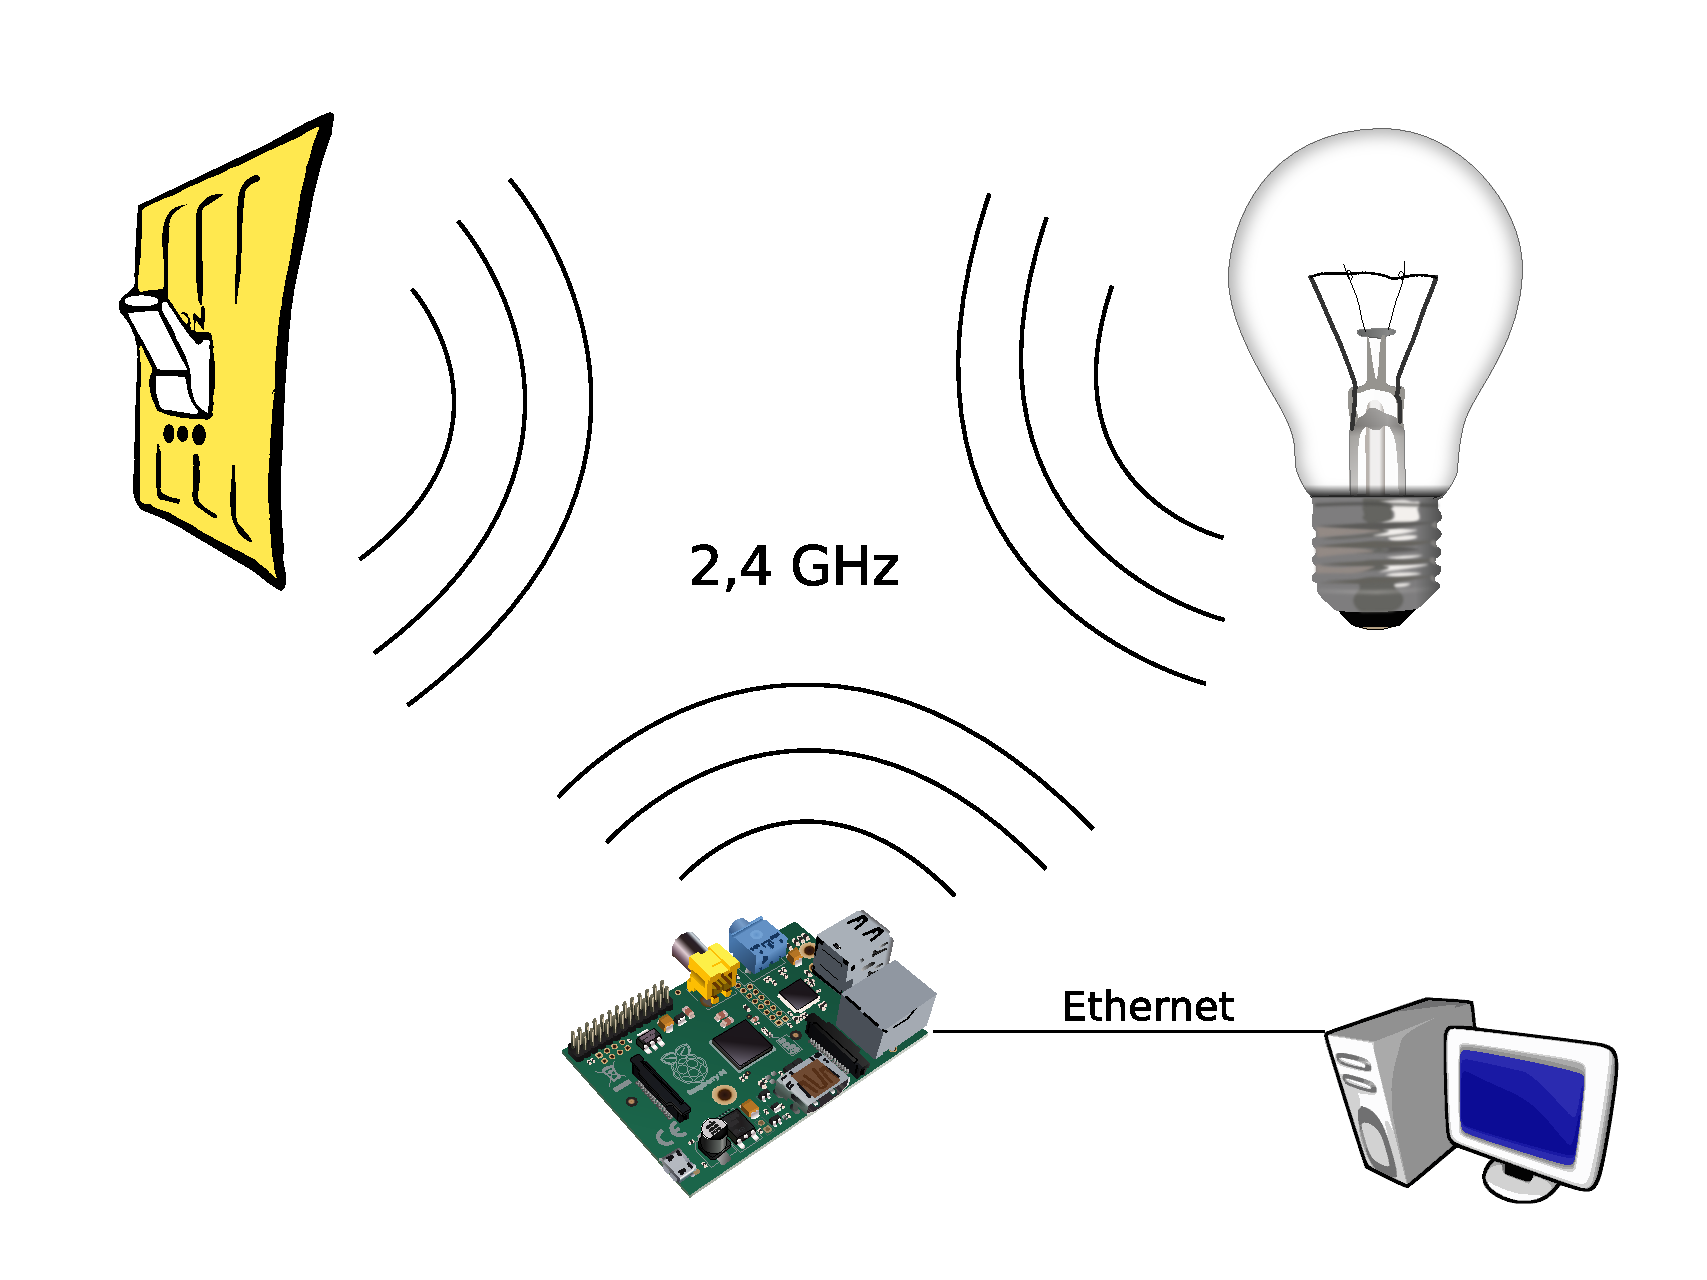
\includegraphics[width=0.5\textwidth]{img/system}
            \caption{Schematische Darstellung der Testumgebung}
            \label{fig:comp}
        \end{figure}

            \begin{itemize}
                \item Ein Aktor kann eine Nachricht mit seiner eigenen Adresse
                    erhalten. Das bedeutet für ihn, er soll diese Aktion
                    ausführen, unabhängig davon wer das Ereignis ausgelöst hat.
                \item Ein Aktor kann programmiert werden auf bestimmte andere
                    Adressen und Nachrichten zu reagieren.
                    So kann beispielsweise eingestellt werden, dass ein Aktor
                    dann schaltet, wenn er eine Nachricht entdeckt, in der steht
                    \enquote{Ich bin Knoten A und meine erste Taste
                    wurde gedrückt} (siehe oben).
            \end{itemize}

            Durch diese zwei Varianten ist es auf der einen Seite möglich,
            dezentral Nachrichten auszulösen und darauf zu reagieren, wobei
            die Auslöser, also die Sensoren selbst relativ einfach aufgebaut
            sein können. Die aufwändigere Logik, welcher Sensor welche Aktion
            auslöst, kann im Aktor implementiert werden.
            Auf der anderen Seite ist es aber trotzdem möglich, das System
            zentral zu nutzen, indem Sensornachrichten von einem zentralen
            Punkt empfangen werden, der anschließend Nachrichten mit konkreten
            Aktoradressen versendet.
            Dies könnte z.\,B. ein Gateway in ein IP-basiertes Netz sein, sodass
            Schaltvorgänge aus dem Internet ausgelöst werden können.
            So können auch Aktoren \enquote{dumm}
            bleiben und können (z.\,B. in einem sehr kleinen, temporären Aufbau)
            ohne jede Programmierung verwendet werden, ohne dass sie von den
            konkreten Sensoren wissen müssen.

\comment / *
\section*{Abkürzungen}
\renewcommand{\IEEEiedlistdecl}{\IEEEsetlabelwidth{CSMA/CA}}
\begin{acronym}
    \acro{6LoWPAN}{IPv6 over Low power Wireless Personal Area Network}
    \acro{CSMA/CA}{Carrier Sense Multiple Access with Collision Avoidance\acroextra{\newline \emph{dt.}: Mehrfachzugriff mit Trägerprüfung und Kollisionsvermeidung}}
    \acro{DIY}{Do-It-Yourself}
    \acro{HAL}{Hardware Abstraction Layer}
    \acro{LAN}{Local Area Network}
    \acro{openHAB}{open Home Automation Bus}
\end{acronym}
\renewcommand{\IEEEiedlistdecl}{\relax}% remember to reset \IEEEiedlistdecl
* /

\comment / *
\listoffigures
\clearpage

\listoftables
\clearpage
* /


\bibliographystyle{IEEEtran}
\bibliography{IEEEabrv,projektdoku_cowbus}

\end{document}
